\documentclass[aspectratio=169,dvipdfmx,xcolor=dvipsnames]{beamer}

% フォント
% 和文の既定フォントをゴシックに変更
\renewcommand{\kanjifamilydefault}{\gtdefault}
% Beamerによる数式フォントの置き換えを阻止
\usefonttheme{professionalfonts} 

% フォントの太さ
\usepackage[deluxe]{otf}
\usepackage[noalphabet]{pxchfon}
\setboldgothicfont{HaranoAjiGothic-Medium.otf} %\bfseriesの設定

% 色
\usepackage{color}
\usetheme{SimplePlus}
\definecolor{dkgreen}{rgb}{0,0.6,0}
\definecolor{gray}{rgb}{0.5,0.5,0.5}
\definecolor{mauve}{rgb}{0.58,0,0.82}

\usepackage{url}

% 数式
\usepackage{amsmath,amsfonts,amsthm,ascmac}
\usepackage{bm}
% 画像
\usepackage{graphicx}
 
% コード
\usepackage{listings}

%ここからソースコードの表示に関する設定
\lstset{
  basicstyle={	tfamily},
  identifierstyle={\small},
  commentstyle={\smallitshape},
  keywordstyle={\small\bfseries},
  ndkeywordstyle={\small},
  stringstyle={\small	tfamily},
  frame={tb},
  breaklines=true,
  columns=[l]{fullflexible},
  numbers=left,
  xrightmargin=0zw,
  xleftmargin=3zw,
  numberstyle={\scriptsize},
  stepnumber=1,
  numbersep=1zw,
  lineskip=-0.5ex
}

\lstset{frame=tb,
  language=Python,
  aboveskip=3mm,
  belowskip=3mm,
  showstringspaces=false,
  columns=flexible,
  basicstyle={\small	tfamily},
  numbers=none,
  numberstyle=	iny\color{gray},
  keywordstyle=\color{blue},
  commentstyle=\color{dkgreen},
  stringstyle=\color{mauve},
  breaklines=true,
  breakatwhitespace=true,
  tabsize=3
}
%ここまでソースコードの表示に関する設定

% 定理環境について
\theoremstyle{definition}
\newtheorem{thm}{定理}
\newtheorem*{thm*}{定理}

\theoremstyle{definition}
\newtheorem{dfn}{定義}

\theoremstyle{definition}
\newtheorem{prop}{命題}
\newtheorem*{prop*}{命題}

\theoremstyle{definition}
\newtheorem{lem}{補題}
\newtheorem*{lem*}{補題}

% 目次の番号を見えなくする設定
\setbeamertemplate{section in toc}{\leavevmode\leftskip=1.75ex
   \kern1.25ex\inserttocsection\par
}
 
%----------------------------------------------------------------------------------------
%	TITLE PAGE
%----------------------------------------------------------------------------------------

\title[short title]{pysparkへの招待} % The short title appears at the bottom of every slide, the full title is only on the title page
\subtitle{}

\author{上野孝斗}

\institute[NTU] % Your institution as it will appear on the bottom of every slide, maybe shorthand to save space
{
    株式会社ネットプロテクションズ \\
    関西開発インターン生\\
    % Your institution for the title page
}
\date{\today} % Date, can be changed to a custom date
\begin{document}

\begin{frame}
  \maketitle
\end{frame}

\begin{frame}{}
  \tableofcontents
\end{frame}

\section{自己紹介}
\begin{frame}
  \begin{itemize}
    \item 所属:関西開発インターン
    \item 担当業務:AFTEE
    \item 大学の専攻:データサイエンス
    \item 所属ゼミで勉強している内容:強化学習,ベイズ統計(聴講)
  \end{itemize}
  \,\,\,\,\,\,\,\,
  \begin{figure}
    \begin{tabular}{cc}
      \begin{minipage}{0.45\hsize}
        \centering
        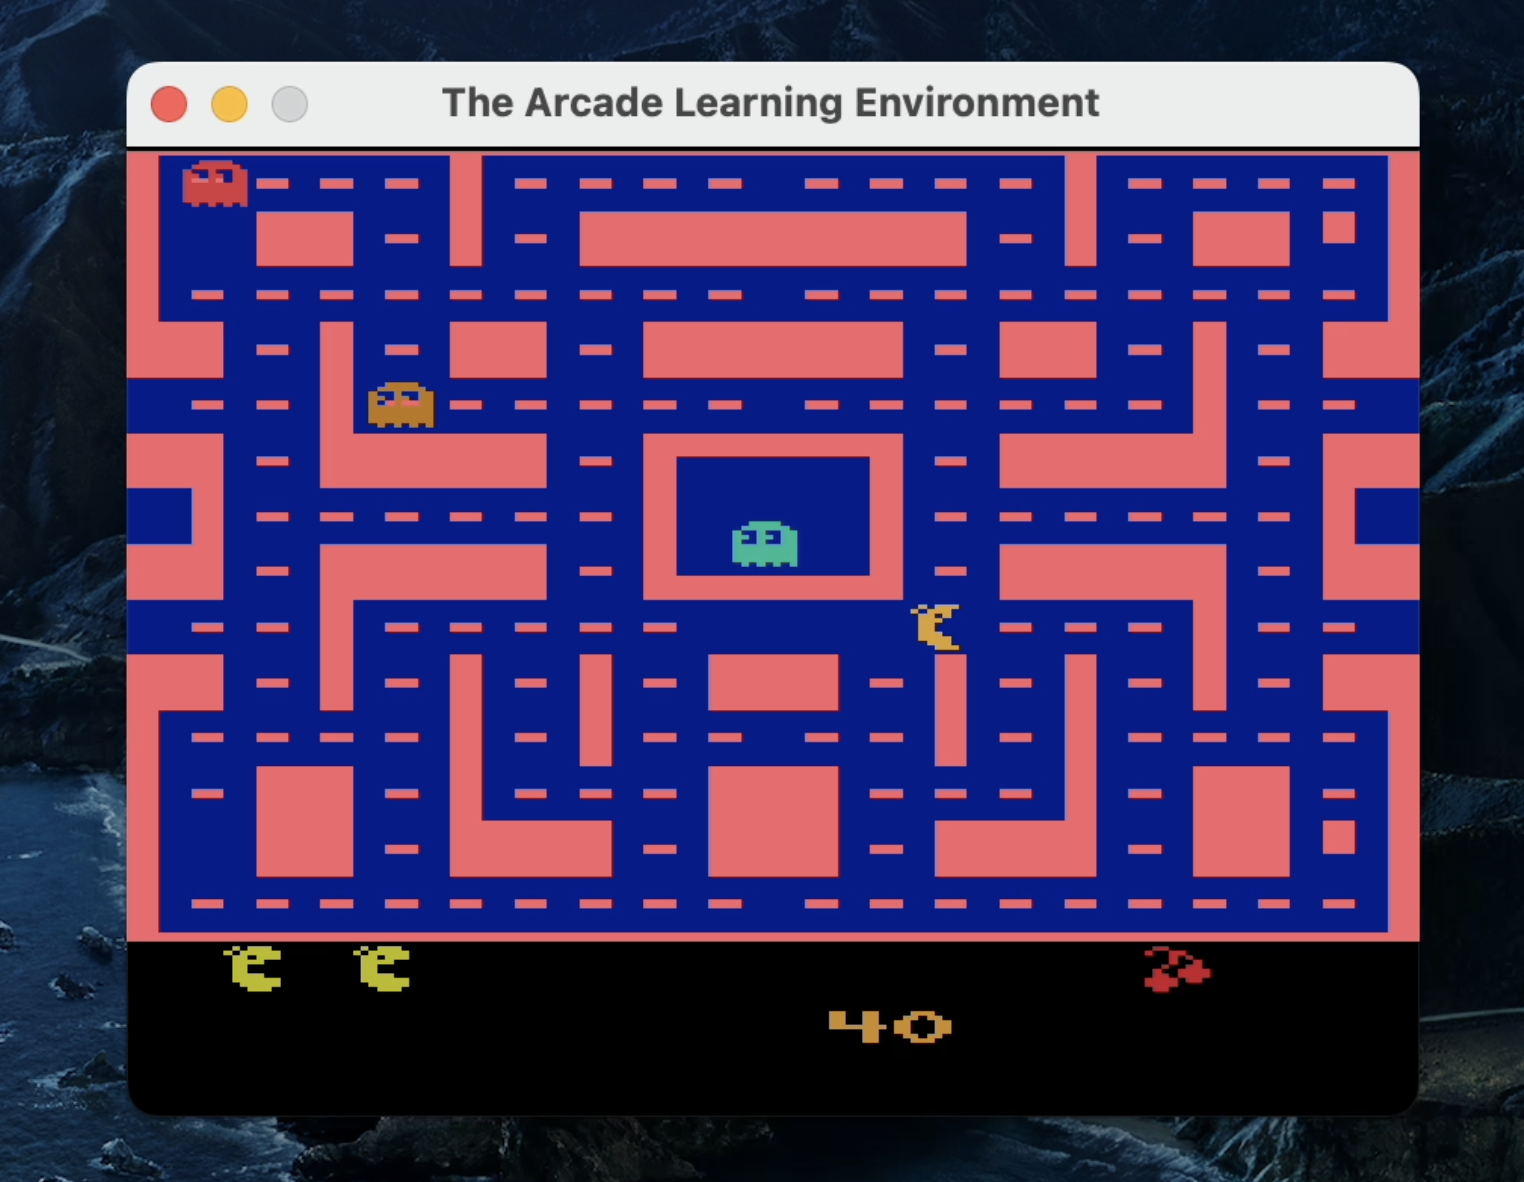
\includegraphics[scale=0.12]{Pacman.png}
      \end{minipage} &
      % ---
      \begin{minipage}{0.45\hsize}
        \centering
        
\includegraphics[scale=0.12]{morimura.png}
      \end{minipage}
      % ---
    \end{tabular}
  \end{figure}

\end{frame}

\section*{pysparkとは?}

\begin{frame}
  \cite{noauthor_pyspark_nodate}にあるちょ
\end{frame}

\begin{frame}
  \bibliographystyle{jplain}
  \bibliography{ref.bib}


\end{frame}

\end{document}